\documentclass{article}
\usepackage{tikz}
\usepackage{amsmath}
\usepackage[paperwidth=26cm,paperheight=12cm,margin=0.3cm]{geometry}
\pagestyle{empty}
\begin{document}
\centering
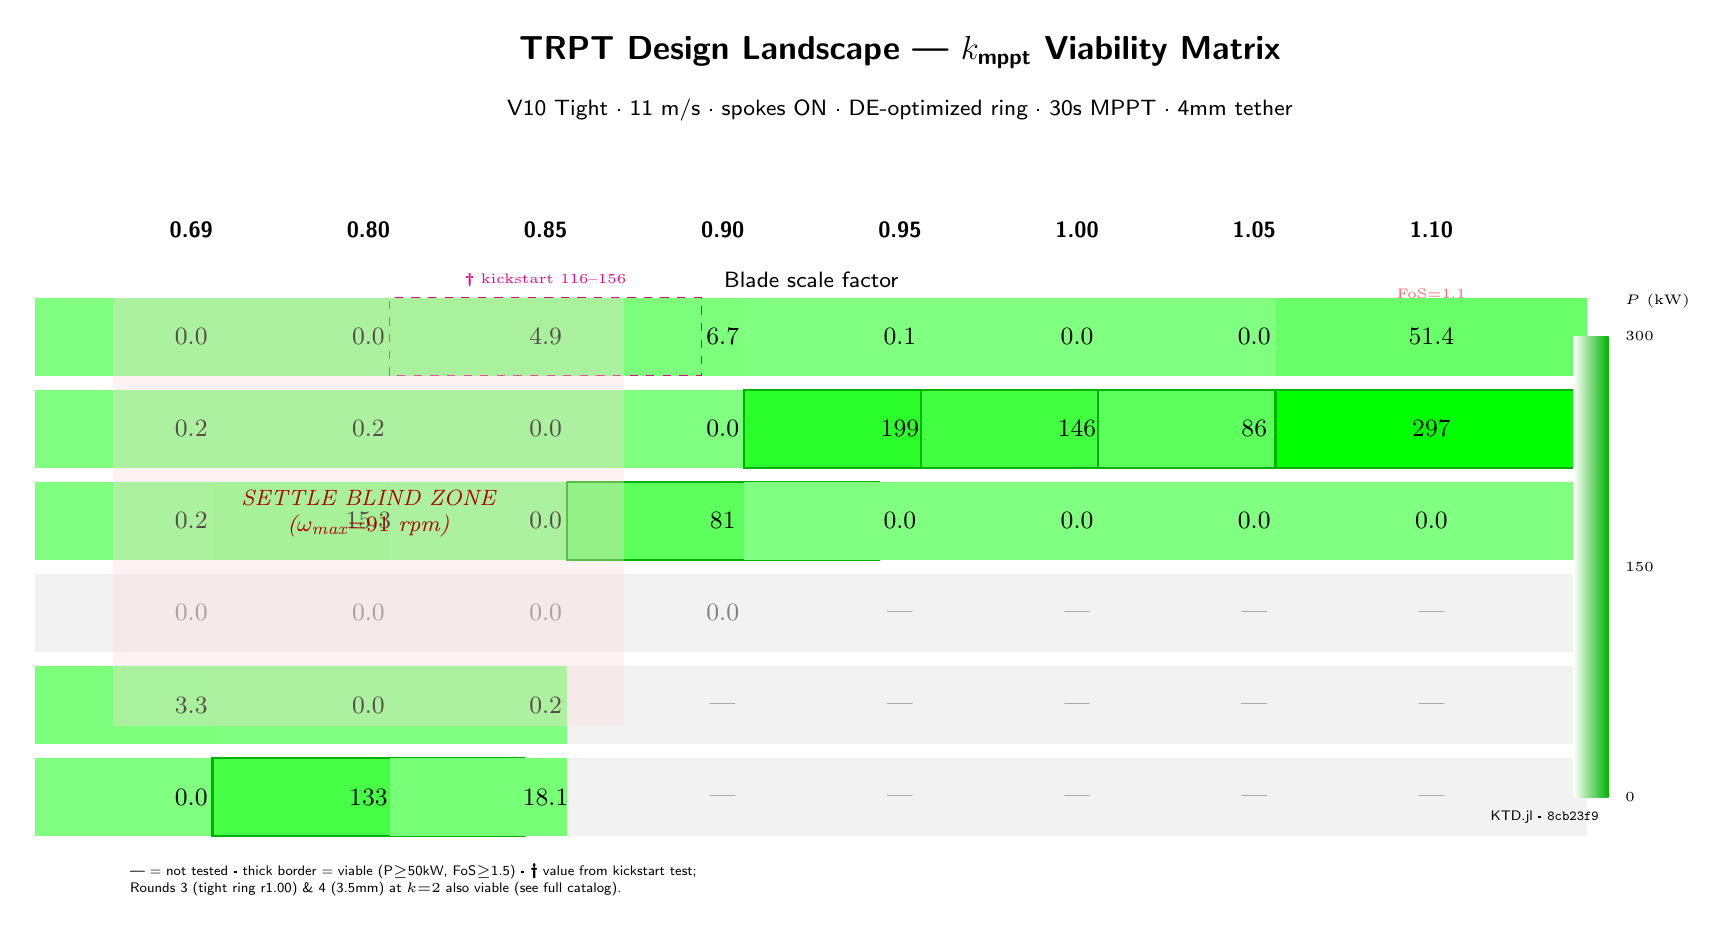
\begin{tikzpicture}[scale=0.9]

% ── Title ──
\node[font=\large\sffamily\bfseries] at (12.0, 12.5) {TRPT Design Landscape — $k_{\text{mppt}}$ Viability Matrix};
\node[font=\footnotesize\sffamily] at (12.0, 11.7) {V10 Tight · 11 m/s · spokes ON · DE-optimized ring · 30s MPPT · 4mm tether};

% Column headers
\foreach \b/\x in {0.69/2.0, 0.80/4.5, 0.85/7.0, 0.90/9.5, 0.95/12.0, 1.00/14.5, 1.05/17.0, 1.10/19.5} {
  \node[font=\footnotesize\sffamily\bfseries] at (\x, 10.0) {\b};
}
\node[font=\footnotesize\sffamily] at (10.75, 9.3) {Blade scale factor};

% Row labels
\foreach \k/\y in {2/8.5, 4/7.2, 6/5.9, 8/4.6, 10/3.3, 14/2.0} {
  \node[font=\small\sffamily, anchor=east] at (0.8, \y) {$k{=}\k$};
}

\def\cw{2.2}
\def\ch{0.55}

% Simple cell: fill with gray or green, draw value, optionally add thick border
% #1=x, #2=y, #3=value, #4=fill_pct (0-100), #5=viable(1/0)
\newcommand{\cv}[5]{
  \ifnum#5=1
    \fill[green!#4!white] (#1-\cw, #2-\ch) rectangle (#1+\cw, #2+\ch);
    \draw[green!70!black, thick] (#1-\cw, #2-\ch) rectangle (#1+\cw, #2+\ch);
  \else
    \pgfmathsetmacro{\f}{#4}
    \fill[green!\f!white] (#1-\cw, #2-\ch) rectangle (#1+\cw, #2+\ch);
  \fi
  \node[font=\small] at (#1, #2) {#3};
}

% Dashed cell (gray bg)
\newcommand{\cd}[3]{
  \fill[gray!10] (#1-\cw, #2-\ch) rectangle (#1+\cw, #2+\ch);
  \node[font=\small, gray] at (#1, #2) {#3};
}

% ── k=2 row ──
\cv{2.0}{8.5}{0.0}{50}{0}
\cv{4.5}{8.5}{0.0}{50}{0}
\cv{7.0}{8.5}{4.9}{51}{0}
\cv{9.5}{8.5}{6.7}{51}{0}
\cv{12.0}{8.5}{0.1}{50}{0}
\cv{14.5}{8.5}{0.0}{50}{0}
\cv{17.0}{8.5}{0.0}{50}{0}
\cv{19.5}{8.5}{51.4}{59}{0}
% Annotations
\node[font=\tiny, magenta] at (7.0, 9.3) {\textbf{†} kickstart 116–156};
\draw[magenta, dashed] (7.0-2.2, 8.5-0.55) rectangle (7.0+2.2, 8.5+0.55);
\node[font=\tiny, red!60] at (19.5, 9.1) {FoS=1.1};

% ── k=4 row ──
\cv{2.0}{7.2}{0.2}{50}{0}
\cv{4.5}{7.2}{0.2}{50}{0}
\cv{7.0}{7.2}{0.0}{50}{0}
\cv{9.5}{7.2}{0.0}{50}{0}
\cv{12.0}{7.2}{199}{83}{1}
\cv{14.5}{7.2}{146}{74}{1}
\cv{17.0}{7.2}{86}{64}{1}
\cv{19.5}{7.2}{297}{100}{1}

% ── k=6 row ──
\cv{2.0}{5.9}{0.2}{50}{0}
\cv{4.5}{5.9}{15.3}{53}{0}
\cv{7.0}{5.9}{0.0}{50}{0}
\cv{9.5}{5.9}{81}{64}{1}
\cv{12.0}{5.9}{0.0}{50}{0}
\cv{14.5}{5.9}{0.0}{50}{0}
\cv{17.0}{5.9}{0.0}{50}{0}
\cv{19.5}{5.9}{0.0}{50}{0}

% ── k=8 row ──
\cd{2.0}{4.6}{0.0}
\cd{4.5}{4.6}{0.0}
\cd{7.0}{4.6}{0.0}
\cd{9.5}{4.6}{0.0}
\cd{12.0}{4.6}{—}
\cd{14.5}{4.6}{—}
\cd{17.0}{4.6}{—}
\cd{19.5}{4.6}{—}

% ── k=10 row ──
\cv{2.0}{3.3}{3.3}{51}{0}
\cv{4.5}{3.3}{0.0}{50}{0}
\cv{7.0}{3.3}{0.2}{50}{0}
\cd{9.5}{3.3}{—}
\cd{12.0}{3.3}{—}
\cd{14.5}{3.3}{—}
\cd{17.0}{3.3}{—}
\cd{19.5}{3.3}{—}

% ── k=14 row ──
\cv{2.0}{2.0}{0.0}{50}{0}
\cv{4.5}{2.0}{133}{72}{1}
\cv{7.0}{2.0}{18.1}{53}{0}
\cd{9.5}{2.0}{—}
\cd{12.0}{2.0}{—}
\cd{14.5}{2.0}{—}
\cd{17.0}{2.0}{—}
\cd{19.5}{2.0}{—}

% ── Settle blind zone overlay ──
\fill[red!15, opacity=0.35] (0.9, 3.0) rectangle (8.1, 9.05);
\node[font=\footnotesize\itshape, red!70!black, align=center] at (4.5, 6.0) {SETTLE BLIND ZONE\\($\omega_{\text{max}}{=}91$ rpm)};

% ── Colorbar ──
\fill[left color=white, right color=green!70!black] (21.5, 2.0) rectangle (22.0, 8.5);
\node[font=\tiny, anchor=west] at (22.1, 2.0) {0};
\node[font=\tiny, anchor=west] at (22.1, 5.25) {150};
\node[font=\tiny, anchor=west] at (22.1, 8.5) {300};
\node[font=\tiny, anchor=west] at (22.1, 9.0) {$P$ (kW)};

% ── Footnote ──
\node[font=\tiny\sffamily, align=left, anchor=north west] at (1.0, 1.2) {
  — = not tested · thick border = viable (P$\ge$50kW, FoS$\ge$1.5) · † value from kickstart test;\\
  Rounds 3 (tight ring r1.00) \& 4 (3.5mm) at $k{=}2$ also viable (see full catalog).
};

% ── Data box ──
\node[font=\tiny\sffamily, anchor=south east] at (22.0, 1.5) {KTD.jl · \texttt{8cb23f9}};

\end{tikzpicture}
\end{document}
